\documentclass[a4paper, 10pt, final, garamond]{book}
\usepackage{cours-preambule}

\raggedbottom

\makeatletter
\renewcommand{\@chapapp}{Induction -- chapitre}
% \renewcommand\thechapter{1 et 2}
\makeatother

\begin{document}
\setcounter{chapter}{3}

\chapter{TD~: Conversion de puissance électromécanique}

\section{Haut parleur «~de \textsc{Laplace}~»}
\label{sec:hplap}
\noindent
\begin{minipage}[t]{.65\linewidth}
	On s'intéresse dans cet exercice à un modèle très simplifié de haut-parleur,
	dans une configuration proche des rails de \textsc{Laplace} où la membrane du
	haut-parleur est fixée solidairement à la tige mobile, qui est également
	reliée élastiquement à un bâti. La tige mobile a pour longueur $\mathrm{AA'} =
		a$, et sa position est repérée par son abscisse $x$, dont l'origine correspond
	à la position de repos. Les frottements de l'air sur la membrane se traduisent
	par une force de frottement linéaire $\vv{f} = -\alpha \vv{v} = -\alpha \xp\,
		\ex$. Le système est forcé électriquement par la tension de commande $u_0$. On
	note $R$ la résistance électrique de l'ensemble, et on néglige
	l'auto-induction.
\end{minipage}
\hfill
\begin{minipage}[t]{.3\linewidth}
	~
	\vspace*{-20pt}
	\begin{center}
		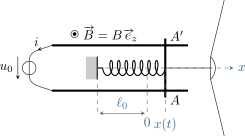
\includegraphics[width=\linewidth]{hplap}
		\captionof{figure}{Schéma du haut-parleur.}
		\label{fig:hplap}
	\end{center}
\end{minipage}
\begin{enumerate}
	\item Exprimer la f.é.m.\ induite en fonction de $\xp$.
	\item Écrire les équations électrique et mécanique.
	\item Découpler ces équations pour aboutir à une unique équation
	      différentielle portant sur la position $x$ de la tige mobile. Quel type
	      d'équation obtient-on~? L'analyser physiquement~: comment se traduisent
	      les phénomènes d'induction~? Commenter leur signe.
	\item Procéder à un bilan de puissance du système et interpréter physiquement
	      chaque terme.
\end{enumerate}

\section{Moteur synchrone}
\label{sec:motsync}
Considérons un modèle simple de moteur synchrone. Le rotor, de moment magnétique
$\vv{m}$, tourne avec la même vitesse angulaire $\w$ constante que le champ
magnétique $\vv{B}$ qui l'entraîne. On néglige tout frottement interne au
moteur. On s'intéresse à l'angle interne du moteur $\tt$ orienté de $\vv{m}$
vers $\vv{B}$ et au couple $\vv{\Gamma}$ exercé par le champ sur le moment
magnétique. On prendra $B = \SI{0.2}{T}$, $m = \SI{8}{A.m^2}$ et une fréquence
de rotation de 50 tours par seconde.
\begin{enumerate}
	\item Proposer un dispositif simple permettant de réaliser le champ magnétique
	      tournant.
	\item Que vaut $\tt$ si le moteur fonctionne à vide~?
	\item Le moteur doit entraîner une charge mécanique qui exerce un couple
	      résistance $\Gamma_r = \SI{0.65}{N.m}$. Calculer l'angle interne et la
	      puissance mécanique fournie par le moteur. D'où provient cette puissance~?
	\item La vitesse de rotation dépend-elle de la charge~? Quel est le couple
	      maximal que peut fournir ce moteur~?
\end{enumerate}

\section{Moteur asynchrone}
\label{sec:motasync}
Le bobinage du rotor d'une machine asynchrone peut être modélisé par une spire
unique de résistance $R$, d'inductance $L$ et de surface $S$ tournant à vitesse
angulaire constante $\w$ autour d'un axe $(\Or x)$. La normale $\vv{n}$ à la
spire est contenue dans le plan $(\O yz)$. Cette spire est plongée dans un champ
$\vv{B}$ généré par le stator, localement uniforme, contenu dans le plan $(\Or
	yz)$, de norme constante, tournant à vitesse angulaire constante $\w'$ autour de
$(\Or x)$. Ce dispositif est utilisé en moteur électrique~: le champ magnétique
entraîne le rotor.
\begin{figure}[h!]
	\centering
	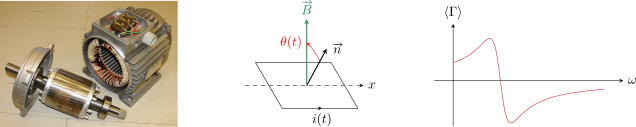
\includegraphics[scale=1]{motasync}
	\caption{Photo, schéma de principe et allure de $\moy{\Gamma}$.}
	\label{fig:motasync}
\end{figure}
\begin{enumerate}
	\item Expliquer \textbf{qualitativement} pourquoi la spire tourne. Les deux
	      vitesses $\w$ et $\w'$ peuvent-elle être identiques~?
	\item Pour simplifier, on suppose qu'à l'instant initial $\vv{n}$ et $\vv{B}$
	      sont colinéaires et de même sens selon $\ez$. Exprimer l'angle $\tt$ en
	      fonction de $\Omega = \w'-\w$. Que représente physiquement la vitesse de
	      glissement $\Omega$~?
	\item Établir l'équation différentielle régissant l'évolution du courant dans
	      le rotor en fonction de $\Omega$.
	\item On se place en régime permanent. Déterminer la pulsation du courant dans
	      la bobine et résoudre l'équation différentielle obtenue précédemment à
	      l'aide de la représentation complexe. Écrire la solution comme une somme
	      de sinus et cosinus.
	\item En considérant le moment magnétique $\vv{m}$ de la spire, calculer le
	      couple auquel elle est soumise. En déduire le couple moyen $\moy{\Gamma}$
	      s'exerçant sur la bobine.
	\item L'allure de la courbe représentant $\moy{\Gamma}$ en fonction de $\w$
	      est donnée ci-dessus. Le moteur peut-il démarrer seul~?
	\item Le moteur doit entraîner une charge mécanique exerçant un couple
	      résistant $\Gamma_r$ connu. Justifier graphiquement qu'un ou deux points
	      de fonctionnement, c'est-à-dire une ou deux vitesses de rotation $\w$,
	      sont possibles. En raisonnant en termes de stabilité par rapport à
	      $\Gamma_r$, justifier qu'un de ces deux points de fonctionnement n'est
	      pas utilisable en pratique~: lequel et pourquoi~?
\end{enumerate}

\section{Oscillateur amorti par induction}
\label{sec:oscamorind}
\noindent
\begin{minipage}[t]{.70\linewidth}
	Considérons une barre de masse $m$ et de longueur $a$, suspendue à deux
	ressorts conducteurs identiques de raideur $k$ et de longueur à vide $\ell_0$.
	L'ensemble est plongé dans un champ magnétique $\vv{B} = B_0\ey$. La barre,
	les ressorts et le support forment un circuit fermé.
	\begin{enumerate}
		\item Établir l'expression du mouvement sur la position $z(t)$ de la barre.
		\item Réaliser et interpréter le bilan de puissance.
		\item À l'instant $t = 0$, on écarte la barre de sa position initiale d'une
		      distance $b$. Déterminer $z(t)$ et $i(t)$.
	\end{enumerate}
\end{minipage}
\hfill
\begin{minipage}[t]{.25\linewidth}
	~
	\vspace*{-10pt}
	\begin{center}
		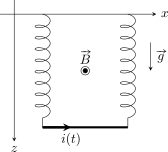
\includegraphics[scale=1]{oscamorind}
		\captionof{figure}{Schéma de la situation.}
		\label{fig:oscamorind}
	\end{center}
\end{minipage}

\section{Rails de \textsc{Laplace} inclinés}
\label{sec:rlplincl}
\noindent
\begin{minipage}[t]{.6\linewidth}
	Un barreau métallique de masse $m$ glisse sans frottement mécanique sur deux
	rails conducteurs, séparés d'une distance $a$ et inclinés d'un angle $\alpha$
	par rapport à l'horizontale. Les rails sont fermés sur une résistance $R$, et
	un champ magnétique uniforme $\vv{B}$, dirigé selon la verticale ascendante,
	règne entre eux. On repère par $x (t)$ la position du barreau le long des
	rails.
	\begin{enumerate}
		\item En appliquant la loi de \textsc{Lenz}, donner le sens du courant $i$ qui
		      circule dans le circuit. La force de \textsc{Laplace} accélère-t-elle ou
		      freine-t-elle la chute du barreau~? Pourrait-il s'immobiliser~?
	\end{enumerate}
\end{minipage}
\hfill
\begin{minipage}[t]{.35\linewidth}
	~
	\vspace*{-10pt}
	\begin{center}
		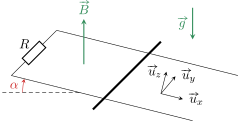
\includegraphics[scale=1]{rlplincl2}
		\captionof{figure}{Schéma des rails.}
		\label{fig:rlplincl2}
	\end{center}
\end{minipage}
\begin{enumerate}[start=2]
	\item Exprimer la force de \textsc{Laplace} $\vv{F_L}$ qui s'exerce sur le
	      barreau mobile en fonction de $i$, $a$, $B$ et $\alpha$.
	\item En exploitant la conservation de la puissance, obtenir une relation en
	      $i$, $R$, $a$, $B$, $\alpha$ et la vitesse $v$ du barreau.
	\item Déterminer l'équation différentielle vérifiée par $v$ et la résoudre,
	      sachant que le barreau est lâché en $x=0$ sans vitesse initiale. Justifier
	      que le mouvement présente un régime transitoire de durée caractéristique
	      $\tau$ à déterminer.
	\item En déduire $x (t)$.
	\item Les rails ont une longueur totale $L$. Déterminer l'énergie électrique
	      totale transmise à la résistance $R$ lors du mouvement du barreau sur les
	      rails, en supposant le temps de chute très grand devant $\tau$.
	      Interpréter.
\end{enumerate}

% \section{Pendule pesant conducteur avec induction}
% \label{sec:pendind}
% \noindent
% \begin{minipage}[t]{.7\linewidth}
% 	On considère un pendule rigide $\rm OA$, homogène, de masse $m$ et de longueur
% 	$\ell$, libre de tourner autour d'un axe vertical $(\Or z)$ passant par une de
% 	ses extrémités. On note $J$ son moment d'inertie par rapport à cet axe. Le
% 	centre de masse $\Gr$ de la tige est situé en son milieu. Le pendule est
% 	repéré par l'angle $\tt$ qu'il forme avec la verticale.
% 	\bigbreak
% 	La tige est en contact en $\rm A$ avec un rail métallique, ce qui forme un
% 	circuit électrique. L'ensemble est placé dans un champ magnétique $\vv{B} =
% 		B\ez$. On ne tient compte que de la résistance $R$ de la tige, et on néglige
% 	celles du rail et du fil servant à fermer le circuit.
% 	\begin{enumerate}
% 		\item Déterminer l'équation différentielle vérifiée par l'angle $\tt$ avec la
% 		      verticale.
% 		\item On suppose les oscillations de petite amplitude. Montrer que si le champ
% 		      magnétique est suffisamment fort, la tige atteint sa position d'équilibre
% 		      sans osciller.
% 		\item Établir un bilan d'énergie et l'analyser qualitativement.
% 	\end{enumerate}
% \end{minipage}
% \hfill
% \begin{minipage}[t]{.2\linewidth}
% 	~
% 	\begin{center}
% 		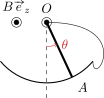
\includegraphics[width=\linewidth]{pendind}
% 		\captionof{figure}{Schéma du pendule.}
% 		\label{fig:pendind}
% 	\end{center}
% \end{minipage}

\end{document}
